\documentclass[professionalfont]{beamer}

\usepackage{graphicx}
\usepackage{newtxtext,newtxmath}
\usetheme{default}
\usecolortheme{seagull}

\setbeamertemplate{navigation symbols}{}
\setbeamertemplate{itemize item}{\textbullet} 
\setbeamertemplate{title page}{
    \begin{center}
        {\textcolor{blue}{\textbf{\fontsize{12}{14}\selectfont ItD: Large Language Models Can Teach Themselves Induction through Deduction}}} \\[1.5cm]
        
        {\fontsize{9}{14}\selectfont Wangtao Sun, et al \\[0.3cm]
        Institute of Automation, Chinese Academy of Sciences \\[0.3cm]
        March 9, 2024}
    \end{center}
}
% ------------------ Title ------------------

\begin{document}
\frame{\titlepage}


\begin{frame}
\begin{center}
    { \textbf{\textcolor{blue}{ {\fontsize{12}{14}\selectfont Abstract} }} }
\end{center}
\\[0.5cm]

{\fontsize{10}{14}\selectfont 
\begin{itemize}
    \item LLMs have limited ability for induction
    
    - Recent researches suggested "Post process"
    
    - But their performance is still limited
\end{itemize}
\\[0.5cm]

\begin{itemize}
    \item New framework: Induction through Deduction
    
    - Deductive Data Generation module
    
    - Naive Bayesian Induction module
\end{itemize}
}

\end{frame}
% ------------------ Slide 1 ------------------

\begin{frame}
\begin{center}
    { \textbf{\textcolor{blue}{ {\fontsize{12}{14}\selectfont Hypothesis search \& Refinement} }} }
\end{center}

{\fontsize{10}{14}\selectfont 
\begin{itemize}
    \item One of recent works
    
    - Weak inductor performs several inductions
    
    - Deductive verification and refinement
\end{itemize}

\begin{itemize}
    \item Inherent induction ability is still limited
    
    - The inductor is weak.
    
    - LLMs are usually good at deduction.
\end{itemize}
}

\begin{center}
    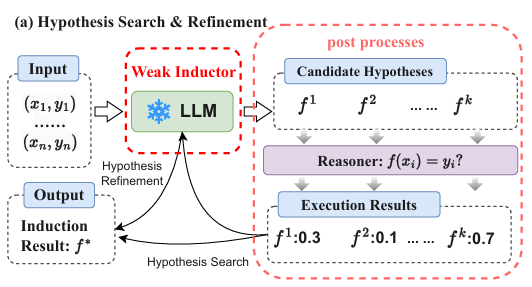
\includegraphics[width=0.7\textwidth]{figure2-1.png}
\end{center}

\end{frame}
% ------------------ Slide 2 ------------------

\begin{frame}
\begin{center}
    { \textbf{\textcolor{blue}{ {\fontsize{12}{14}\selectfont Induction through Deduction} }} }
\end{center}

{\fontsize{10}{14}\selectfont 
\begin{itemize}
    \item Deductive Data Generation module
    
    - Using given samples, generates more samples
    
    - Combined with LoRA, inductor performs induction
\end{itemize}

\begin{itemize}
    \item Naive Bayesian Induction module
    
    - Verify reliability of the generator's augmentation
    
    - Fine-tunes LLM to predict \(p(f|x,y)\) supposing \((x_{i}, y_{i})\) are iid.
\end{itemize}
}

\begin{center}
    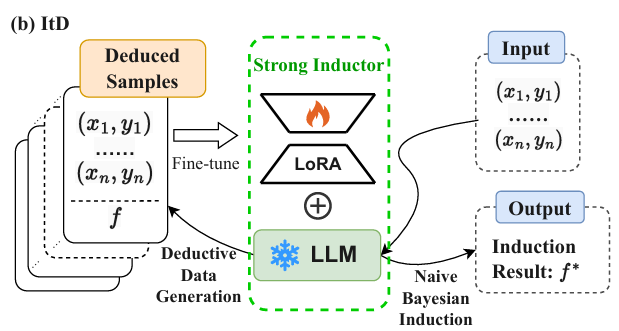
\includegraphics[width=0.7\textwidth]{figure2-2.png}
\end{center}

\end{frame}
% ------------------ Slide 3 ------------------

\begin{frame}
\begin{center}
    { \textbf{\textcolor{blue}{ {\fontsize{12}{14}\selectfont Experiment} }} }
\end{center}

{\fontsize{10}{14}\selectfont 
\begin{itemize}
    \item Instruction Induction Task (Semantic)
    
    - x and y are Natural Language sentences
\end{itemize}

\begin{itemize}
    \item List Function Task (Symbolic)
    
    - x and y are list with numeric data
\end{itemize}
}

\begin{center}
    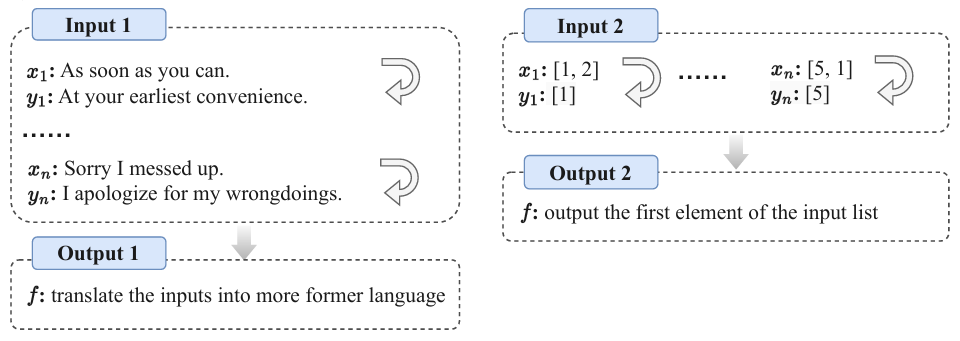
\includegraphics[width=1.0\textwidth]{figure1.png}
\end{center}

\end{frame}
% ------------------ Slide 4 ------------------

\begin{frame}
\begin{center}
    { \textbf{\textcolor{blue}{ {\fontsize{12}{14}\selectfont Conclusion} }} }
\end{center}
\\[0.5cm]

{\fontsize{10}{14}\selectfont 
\begin{itemize}
    \item ItD is superior to existing methods
    
    - ItD achieved improvement of 36\%, 10\% with previous SOTA

    - Improvement of both the semantic, symbolic deduction
\end{itemize}
\\[0.5cm]

\begin{itemize}
    \item Limitation
    
    - Compared to semantic task, symbolic performance was not satisfying
    
    - Naive Bayesian is greedy, leading to local-optima
\end{itemize}
}

\end{frame}
% ------------------ Slide 5 ------------------

\end{document}
